%license:BSD-3-Clause
%copyright-holders:Michele Maione
%============================================================
%
%	Piattaforma di cloud gaming per giochi arcade
%
%============================================================

\chapter{Prestazioni} \label{cap:cap4}
%Si mostra il progetto dal punto di vista sperimentale, le cose materialmente realizzate. In questa sezione si mostrano le attività sperimentali svolte, si illustra il funzionamento del sistema (a grandi linee) e si spiegano i risultati ottenuti con la loro valutazione critica. Bisogna introdurre dati sulla complessità degli algoritmi e valutare l'efficienza del sistema.
Questo capitolo analizza le prestazioni del progetto relativamente ai tre difetti intrinseci del cloud gaming: riduzione della qualità audiovisiva, il problema della latenza ed il bit-rate richiesto.



\section{Riduzione della qualità audiovisiva}
Nell'ambito videoludico la qualità audiovisiva (soprattutto quella visiva) influisce sulla qualità generale percepita dall'utente, per questo nel cloud gaming è necessario garantire un livello di qualità quasi identico alla situazione in cui il gioco viene eseguito in locale. È possibile preservare la qualità percepita durante lo streaming anche se si utilizzano bassi bit-rate, che sono particolarmente adatti per l'utilizzo in reti cellulari e WLAN \parencite{VideoAndMultimediaTransmissionsOverCellularNetworks}.



\subsection{La qualità visiva}
Qualsiasi elaborazione applicata ad un'immagine può causare una perdita di qualità. La qualità dell'immagine si riferisce al modo in cui viene riprodotta la scena ripresa (o quella generata digitalmente) e può essere descritta dal degradarsi di alcune caratteristiche tra cui: nitidezza, gamma dinamica, fusione dei colori, contrasto, sfocatura, ecc\dots. I metodi di valutazione della qualità dell'immagine sono suddivisi in due categorie: soggettivi ed oggettivi. I metodi soggettivi sono composti da test psicofisici per la valutazione, da parte di osservatori, della qualità percepita. Questi test sono dispendiosi in in termini di risorse e di tempo, sia per la preparazione che per l'esecuzione. Le valutazioni vengono poi utilizzate come termini di paragone per i metodi oggettivi \parencite{AnewcombinedPSNRforobjectivevideoqualityassessment}. I metodi oggettivi si basano su confronti utilizzando criteri numerici espliciti. L'errore quadratico medio (MSE), il \textit{peak signal-to-noise ratio} (PSNR) e la \textit{structural similarity index measure} (SSIM) sono esempi di misure di qualità utilizzate nell'analisi delle immagini \parencite{relationship_PSNR_and_SSI}.



\subsubsection{Peak signal-to-noise ratio}
Il PSNR è comunemente usato come misura della qualità della compressione e della riduzione del rumore nelle immagini digitali a scala di grigi. Esistono diversi approcci per calcolare il PSNR delle immagini a colori, ad esempio (il più semplice) utilizzando immagini in formato YCbCr e calcolando il PSNR solo sul canale della luminanza. Il PSNR è espresso solitamente in decibel con valori tipici per la compressione video per lo streaming tra $20$ \si{dB} e $30$ \si{dB} \parencite{ThomosN2006OtoJ} e si calcola utilizzando l'Eq. \ref{eq:PSNR}, con $MSE(f,g)$ l'errore quadratico medio e $L = 255$ l'intervallo dinamico \parencite{AnewcombinedPSNRforobjectivevideoqualityassessment}.

\begin{equation} \label{eq:PSNR}
	PSNR(f,g)=10 \log_{10}  \frac{L^2}{MSE(f,g)}	
\end{equation}



\subsubsection{Structural Similarity Index Measure}
SSIM è un metodo per predirre la qualità percepità nelle immagini digitali. Invece di utilizzare i tradizionali metodi di somma degli errori, SSIM è progettato modellando qualsiasi distorsione dell'immagine come una combinazione di tre fattori: la perdita di correlazione, la distorsione della luminanza e la distorsione del contrasto. L'indice SSIM è un valore decimale compreso tra $0$ e $1$ e si calcola utilizzando l'Eq. \ref{eq:SSIM} con \parencite{relationship_PSNR_and_SSI}:

\begin{itemize}
	\item $k_1 = 0,01$ e $k_2 = 0,03$ costanti;
	\item $L = 255$ l'intervallo dinamico;
	\item $c_1 = (k_1 L)^2$, $c_2 = (k_2 L)^2$ e $c_3 = c_2/2$ variabili di stabilizzazione della divisione;
	\item $l(f,g)$ funzione di comparazione della luminanza tra le medie $\mu_f$ e $\mu_g$;
	\item $c(f,g)$ funzione di comparazione del contrasto tra le deviazioni standard $\sigma_f$ e $\sigma_g$;
	\item $s(f,g)$ funzione di comparazione della struttura che misura il coefficiente di correlazione; $\sigma_{fg}$ è la covarianza tra $f$ e $g$.
\end{itemize}

\begin{equation} \label{eq:SSIM}
	\begin{matrix*}[l]
		SSIM(f,g) =  l(f,g) c(f,g) s(f,g) & l(f,g)= \frac{2 \mu_f \mu_g  + C_1}{\mu_f^2 \mu_g^2  + C_1} \\
		c(f,g)= \frac{2 \sigma_f \sigma_g  + C_2}{\sigma_f^2 + \sigma_g^2  + C_2} & s(f,g)= \frac{\sigma_{fg}+C_3}{\sigma_f \sigma_g + C_3}
	\end{matrix*}
\end{equation}



\subsubsection{Risultati ottenuti}
Tramite lo script in Lis. \ref{lst:PyPSNR_SSIM} è stata calcolata la qualità video per la codifica \textit{MPEG-1 Video} a 1024 kbps che ha dato come risultati un valore di PSNR di $27,703$ \si{dB} e un indice SSIM del $89,9\%$. Alcune immagini d'esempio del risultato ottenuto sono visibili in Fig. \ref{fig:BMP_MPEG_compare}.

\begin{lstlisting}[language=Python, caption=Script Python per il calcolo di PSNR e SSIM, label={lst:PyPSNR_SSIM}]
imgRGB = skimage.io.imread("frameRGB.bmp")
imgMPEG1 = skimage.io.imread("frameMPEG1.bmp")

PSNR = skimage.metrics.peak_signal_noise_ratio(imgRGB, imgMPEG1)

SSIM = skimage.metrics.structural_similarity(imgRGB, imgMPEG1,
	multichannel=True)
\end{lstlisting}

\begin{figure}[H]
	\centering
	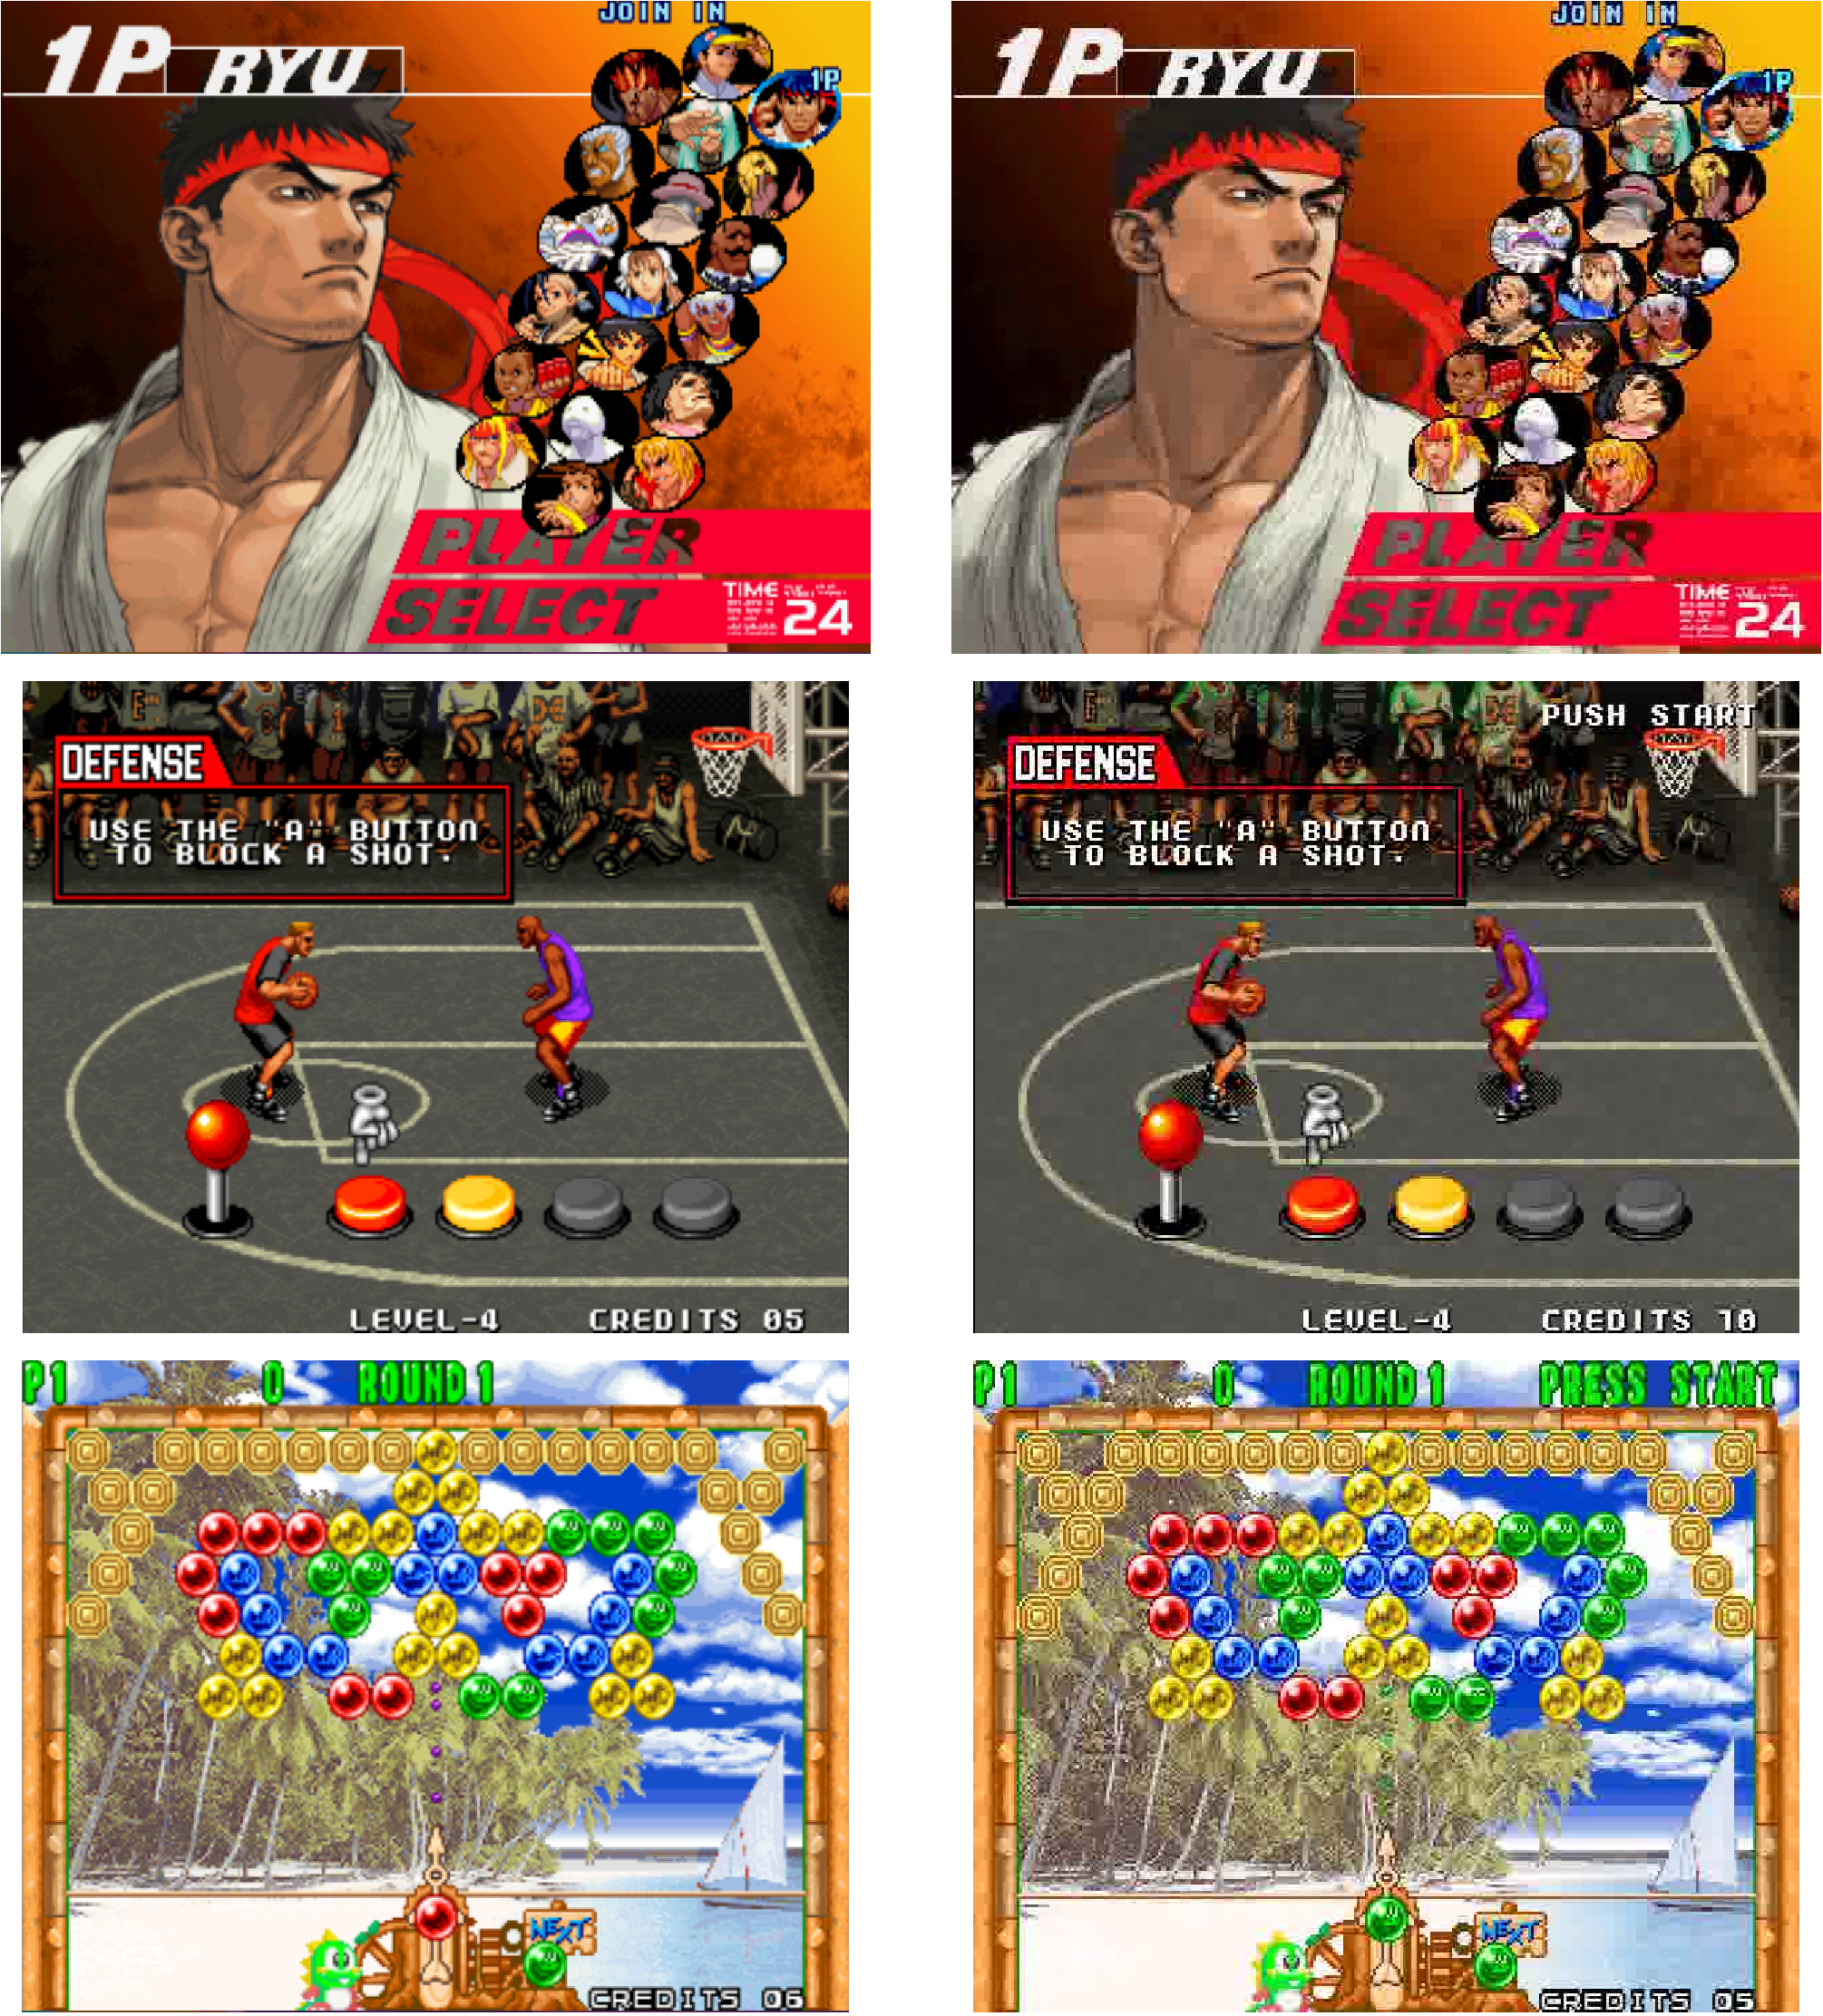
\includegraphics[width=\linewidth]{immagini/BMP_MPEG_compare}
	\caption{Alcuni frame d'esempio: a sinistra i frame renderizzati dal MAME (RGBA), a destra i frame codificati in \textit{MPEG-1}. © Capcom, Data East, Taito}
	\label{fig:BMP_MPEG_compare}
\end{figure}



\subsection{La qualità uditiva}
Gli algoritmi sviluppati per misurare oggettivamente la qualità audio percepita simulano le proprietà percettive dell'orecchio umano ed applicano modelli informatici per stimare le similarità tra due segnali audio. Tra questi algoritmi abbiamo \textit{Perceptual Evaluation of Audio Quality} (PEAQ), \textit{Perceptual Objective Listening Quality Assessment} (POLQA) ed \textit{Evaluation of Audio Quality} (EAQUAL). Questi algoritmi sono brevettati e protetti da licenza ma per PEAQ è disponibile un'implementazione per uso accademico a cura di Giuseppe Gottardi\footnote{Il repository del progetto è disponibile qui: sourceforge.net/projects/peaqb.} \parencite{PoctaPeter2015SaOA}.



\subsubsection{Perceptual Evaluation of Audio Quality}
\textit{Perceptual Evaluation of Audio Quality} (PEAQ) è un algoritmo sviluppato dal ITU-R\footnote{ITU-R: \textit{International Telecommunication Union - Radiocommunication Sector} è un organizzazione internazionale che si occupa degli standard nel campo delle telecomunicazioni, settore radio.} che simula le proprietà percettive dell'orecchio umano tramite modelli informatici, per determinare il livello di rumore che si può introdurre in un segnale acustico prima che esso diventi udibile. Per PEAQ sono stati creati due modelli, \textit{basic} e \textit{advanced}, il modello avanzato viene utilizzato per test più approfonditi \parencite{UlovecK2018PAQA}. Gli output dell'algoritmo sono il \textit{Objective Difference Grade} (ODG) e l'\textit{indice di distorsione} (DI) che vengono assegnati ad ogni frame audio, in questo modo si può intervenire precisamente sull'algoritmo di codifica per migliorarlo. Facendo la media degli ODG di tutti i frame si può dare una stima della qualità di tutto il segnale. La scala ODG è basata su un test uditivo soggettivo (ITU-R BS.1116) ed è la seguente: \textit{molto fastidioso} (1), \textit{fastidioso} (2), \textit{leggermente fastidioso} (3), \textit{percettibile ma non fastidioso} (4), \textit{impercettibile} (5) \parencite{PoctaPeter2015SaOA}.

Il metodo, illustrato in Fig. \ref{fig:PEAQ}, inizia applicando un allineamento temporale tra i due segnali in ingresso (alcuni codificatori slittano leggermente il segnale in avanti), questi vengono inviati al modello percettivo. I segnali audio vengono tagliati in frame di $0,042$ s con una sovrapposizione del $50\%$. Il modello percettivo trasforma i segnali utilizzando una funzione finestra e una \textit{FFT}. Successivamente vengono applicati dei pre-processamenti per calcolare: i modelli di eccitazione, i modelli di volume, i modelli di modulazione e il segnale di errore. Utilizzando questi modelli una funzione calcola le \textit{Model Output Variables} (MOVs) che vengono mappate sul corrispettivo \textit{ODG} \parencite{PEAQ}.

\begin{figure}[H]
	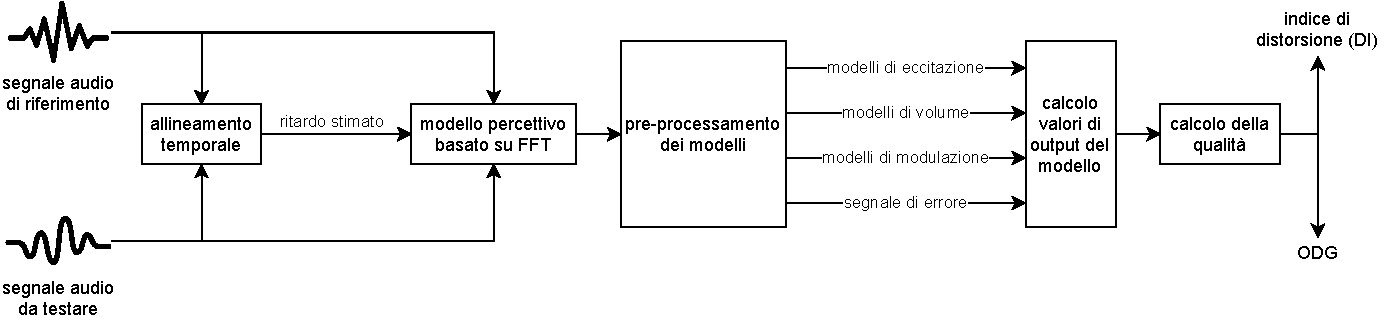
\includegraphics[width=\linewidth]{immagini/PEAQ}
	\caption{Diagramma del funzionamento di PEAQ}	
	\label{fig:PEAQ}
\end{figure}



\subsubsection{Risultati ottenuti}
In questo progetto è stata usata un'implementazione per scopi accademici di PEAQ, con cui è stato calcolato per una partita di 2 minuti di \textit{Street Fighter III}, codificato con \textit{MPEG-1 Audio Layer II} (MP2) a 64 kbps, un grado PEAQ di 2 (\textit{fastidioso}).




\section{Il problema della latenza} \label{sec:cap4_Latenza}
Alle fasi di base di un videogioco (ricezione input, esecuzione, rendering e display) nel cloud gaming vanno ad aggiungersi: invio al server dell'input utente, codifica, trasmissione e decodifica. Queste fasi aggiuntive aumentano il tempo che intercorre tra l'input del giocatore e l'azione visualizzata sullo schermo.

Un leggero ritardo in un film in streaming o in una videochiamata molto probabilmente passa inosservato, ma durante una partita la latenza può rendere il gioco non fruibile, fortunatamente il rapido sviluppo delle reti a banda larga hanno reso questo problema meno evidente. %e il cloud gaming una realtà.

Secondo diversi studi, affinché il gameplay sia fluido e senza jitter\footnote{Il jitter è la variazione del ritardo tra i pacchetti inviati.}, il ritardo tra la trasmissione dell'input utente e la visualizzazione dell'azione corrispondente, chiamato anche \textit{round trip delay}, deve essere inferiore a una soglia tollerabile, altrimenti la reazione dell'utente viene visualizzata con un ritardo che rende il gameplay difficoltoso e irritante, soprattutto nei giochi in cui la velocità è un fattore molto importante, come gli sparatutto in prima persona e i giochi di strategia in tempo reale. In tabella \ref{table:Ritardo_tollerato_per_tipo_di_gioco} sono riportate le soglie di ritardo tollerabili per tipo di gioco \parencite{Cloud_Gaming_Architecture_and_Performance}.

\begin{table}[H]
	\centering
	\begin{tabular}{||l l r||}
		\hline
		Tipo di gioco & Prospettiva & Soglia di ritardo (ms) \\
		\hline\hline
		FPS & Prima persona & 100 \\
		\hline
		RPG & Terza persona & 500 \\
		\hline
		RTS & Onnipresente & 1000 \\
		\hline
	\end{tabular}

	\caption{Ritardo tollerato per tipo di gioco}
	\label{table:Ritardo_tollerato_per_tipo_di_gioco}
\end{table}



\subsubsection{Risultati ottenuti}
La latenza è stata calcolata cronometrando il \textit{round trip delay} e calcolando le medie al termine della partita, lato server della codifica\footnote{Il tempo medio di codifica contiene anche il tempo di cattura.} e della creazione del pacchetto di rete, e lato client della decodifica. Per calcolare il \textit{round trip delay} è stata eseguita una sessione di gioco di \textit{Street Fighter III} ed è stato effettuato lo screencast utilizzando il programma \textit{OBS Studio}\footnote{OBS Studio è un software open-source per lo streaming e la cattura video.} a 60 fps. Utilizzando una \textit{tastiera su schermo} si preme il tasto \textit{P} per mettere il gioco in pausa, e successivamente viene analizzato manualmente lo screencast, calcolando il \textit{round trip delay} medio tra il frame in cui avviene la pressione del tasto e la visualizzazione a video del frame del gioco in pausa\footnote{In MAME il frame di pausa è un frame a cui viene abbassato il canale alfa su sfondo nero.}, come mostrato in Fig. \ref{fig:pause}. Il tempo medio di trasmissione\footnote{Il tempo medio di trasmissione contiene anche il tempo di visualizzazione del frame sullo schermo.} è stato calcolato come la differenza tra il \textit{round trip delay} medio e le altre operazioni. I test sono stati effettuati su rete LAN utilizzando i computer descritti in Tab. \ref{table:ServerUsato} e Tab. \ref{table:ClientUsato}. I tempi medi ottenuti sono mostrati in Tab. \ref{table:LatenzaOttenuta}.

\begin{figure}[H]
	\centering
	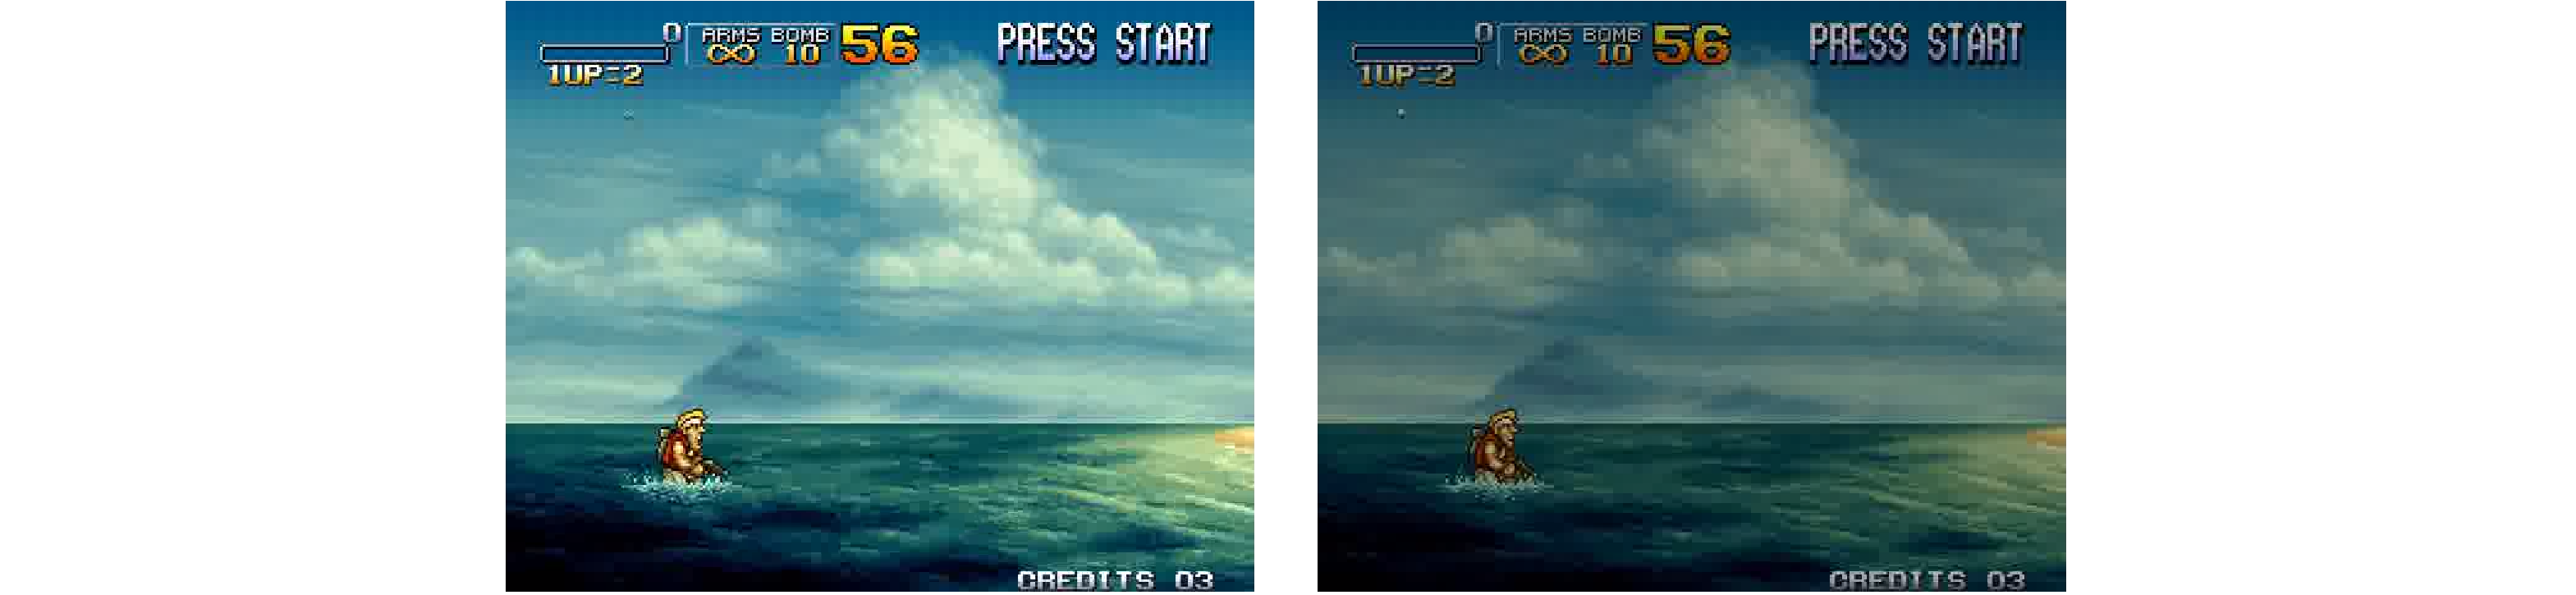
\includegraphics[height=2.3cm]{immagini/pause}
	\caption{Frame di gioco (sx) e frame di pausa (dx). © Capcom}	
	\label{fig:pause}
\end{figure}

\begin{table}[H]
	\centering
	\begin{tabular}{||l r||}
		\hline
		Operazione & Tempo (ms) \\
		\hline\hline
		\hline
		Codifica & $6,71$ \\
		\hline
		Creazione pacchetto di rete & $0,07$ \\
		\hline
		Trasmissione & $\sim 174,00$ \\
		\hline
		Decodifica & $1,04$ \\
		\hline\hline
		\textbf{Round trip delay} & \textbf{$\sim 182,00$} \\
		\hline
	\end{tabular}

	\caption{Tempi medi d'elaborazione per \textit{Street Fighter III}}
	\label{table:LatenzaOttenuta}
\end{table}

Sono stati effettuati dei test per la stima del tempo di \textit{round-trip}\footnote{Con il termine \textit{round-trip} si intende il messaggio che il client invia al server e che il server invia al client. In questo caso viene inviata anche una marca temporale.} da vari comuni italiani utilizzando il server descritto in Tab. \ref{table:ServerUsato}. I risultati ottenuti sono mostrati in Tab. \ref{table:PingPong}.

\begin{table}[H]
	\centering
	\begin{tabular}{||l r r r||}
		\hline
		Comune & Distanza (km) & Min (ms) & Max (ms) \\
		\hline\hline
		\hline		
		Milano (MI) & $\sim1540$ & 20 & 28 \\
		\hline
		Lamezia Terme (CZ) & $\sim740$ & 20 & 40 \\		
		\hline
		Olgiate Olona (VA) & $\sim1620$ & 28 & 38 \\
		\hline
		Bologna (BO) & $\sim1160$ & 30 & 60 \\
		\hline
		Campobasso (CB) & $\sim300$ & 30 & 60 \\
		\hline
		Casalpusterlengo (LO) & $\sim1440$ & 35 & 40 \\		
		\hline
		Treviso (TV) & $\sim1480$ & 35 & 45 \\
		\hline		
		Basiano (MI) & $\sim1580$ & 30 & 50 \\
		\hline
		Verona (VR) & $\sim1420$ & 30 & 70 \\		
		\hline
		Novara (NO) & $\sim1640$ & 30 & 80 \\
		\hline
	\end{tabular}

	\caption{Tempo di \textit{round-trip} da vari comuni italiani}
	\label{table:PingPong}
\end{table}

\begin{table}[H]
	\centering
	\begin{tabular}{||l l||}
		\hline
		Componente & Valore \\
		\hline\hline
		\hline
		CPU & AMD Ryzen 5 2500U (8 threads) @ $3,6$ GHz \\
		\hline
		GPU & AMD Radeon Vega 8 Mobile Graphics $4$ GB \\
		\hline
		RAM & 8 GB \\
		\hline
		Connessione internet & $download 41,5$ mbps, $upload 10,5$ mbps \\
		\hline
		S.O. & Fedora 34 \\
		\hline
		Posizione & Sant'Anastasia (NA) \\
		\hline
	\end{tabular}

	\caption{Server utilizzato per il test}
	\label{table:ServerUsato}
\end{table}

\begin{table}[H]
	\centering
	\begin{tabular}{||l l||}
		\hline
		Componente & Valore \\
		\hline\hline				
		\hline
		CPU & Intel Core2 Quad Q6600 (4 threads) @ $2,4$ GHz \\
		\hline
		GPU & Nvidia GeForce 9500 GT 1 GB\\
		\hline
		RAM & 8 GB \\		
		\hline
		S.O. & Windows 10 \\
		\hline
		Browser & Firefox 88 \\
		\hline
	\end{tabular}

	\caption{Client utilizzato per il test}
	\label{table:ClientUsato}
\end{table}




\section{Bit-rate richiesto}
È necessario stimare il bit-rate richiesto per offrire un'esperienza di gioco all'utente priva di ritardi e con la miglior qualità audiovisiva. Il bit-rate richiesto è l'unico parametro che è influenzato dalla compressione video, e differisce tra i vari giochi. Calcolando i differenti bit-rate massimi per le differenti qualità audiovisive si può scegliere il miglior bilanciamento tra qualità offerta e bit-rate richiesto all'utente \parencite{ChenKuanTa2014OtQo}.

\subsubsection{Risultati ottenuti}
Il MAME CGP può essere avviato specificando la risoluzione video da utilizzare e come mostrato in Tab. \ref{table:PiattaformeDiCloudGaming} è stata usata una risoluzione di 480p, che con la compressione \textit{MPEG-1 Video} ed \textit{MPEG-1 Audio Layer II}, necessitano di un bit-rate medio di 1 Mbps (con picchi in alcuni casi fino a 3.5 Mbps). Utilizzando lo script in Lis. \ref{lst:PyBitRate} sono stati estrapolati i dati mostrati in Tab. \ref{table:bandwidth_e_medie} e Fig. \ref{fig:bandwidth}.

\begin{lstlisting}[language=Python, caption=Script Python per il calcolo del bit-rate richiesto, label={lst:PyBitRate}]
try:
	while True:
		new_value = psutil.net_io_counters().bytes_recv
		new_seconds += 0.1
		seconds.append(new_seconds)

		if old_value
			bw = (new_value - old_value) * 8. / 1024. / 1024.
		else:
			bw = 0

		bandwidth.append(bw)
		old_value = new_value
		time.sleep(0.1)
except KeyboardInterrupt:
	pass

print("Media:", statistics.mean(bandwidth))
print("Dev. std:", statistics.stdev(bandwidth))
print("Varianza:", statistics.variance(bandwidth))
\end{lstlisting}

\begin{table}[H]
	\centering
	\begin{tabular}{||l l r r r||}
		\hline
		Gioco & Tipo & Media & Dev. std & Varianza \\
		\hline\hline
		\hline
		Castelvania & piattaforma & 0.867 & 0.537 & 0.289 \\
		\hline		
		Metal Slug 3 & piattaforma & 0.688 & 0.360 & 0.129 \\
		\hline
		Out Run & guida & 0.835 & 0.443 & 0.196 \\
		\hline
		Puzzle Booble 2 & puzzle & 0.731 & 0.320 & 0.102 \\
		\hline
		Street Fighter III & picchiaduro & 0.848 & 0.400 & 0.160 \\
		\hline	
		Street Slam & sport & 1.075 & 0.555 & 0.308 \\
		\hline
	\end{tabular}

	\caption{Bit-rate richiesto per vari tipi di giochi (in Mbps)}
	\label{table:bandwidth_e_medie}
\end{table}

\begin{figure}
	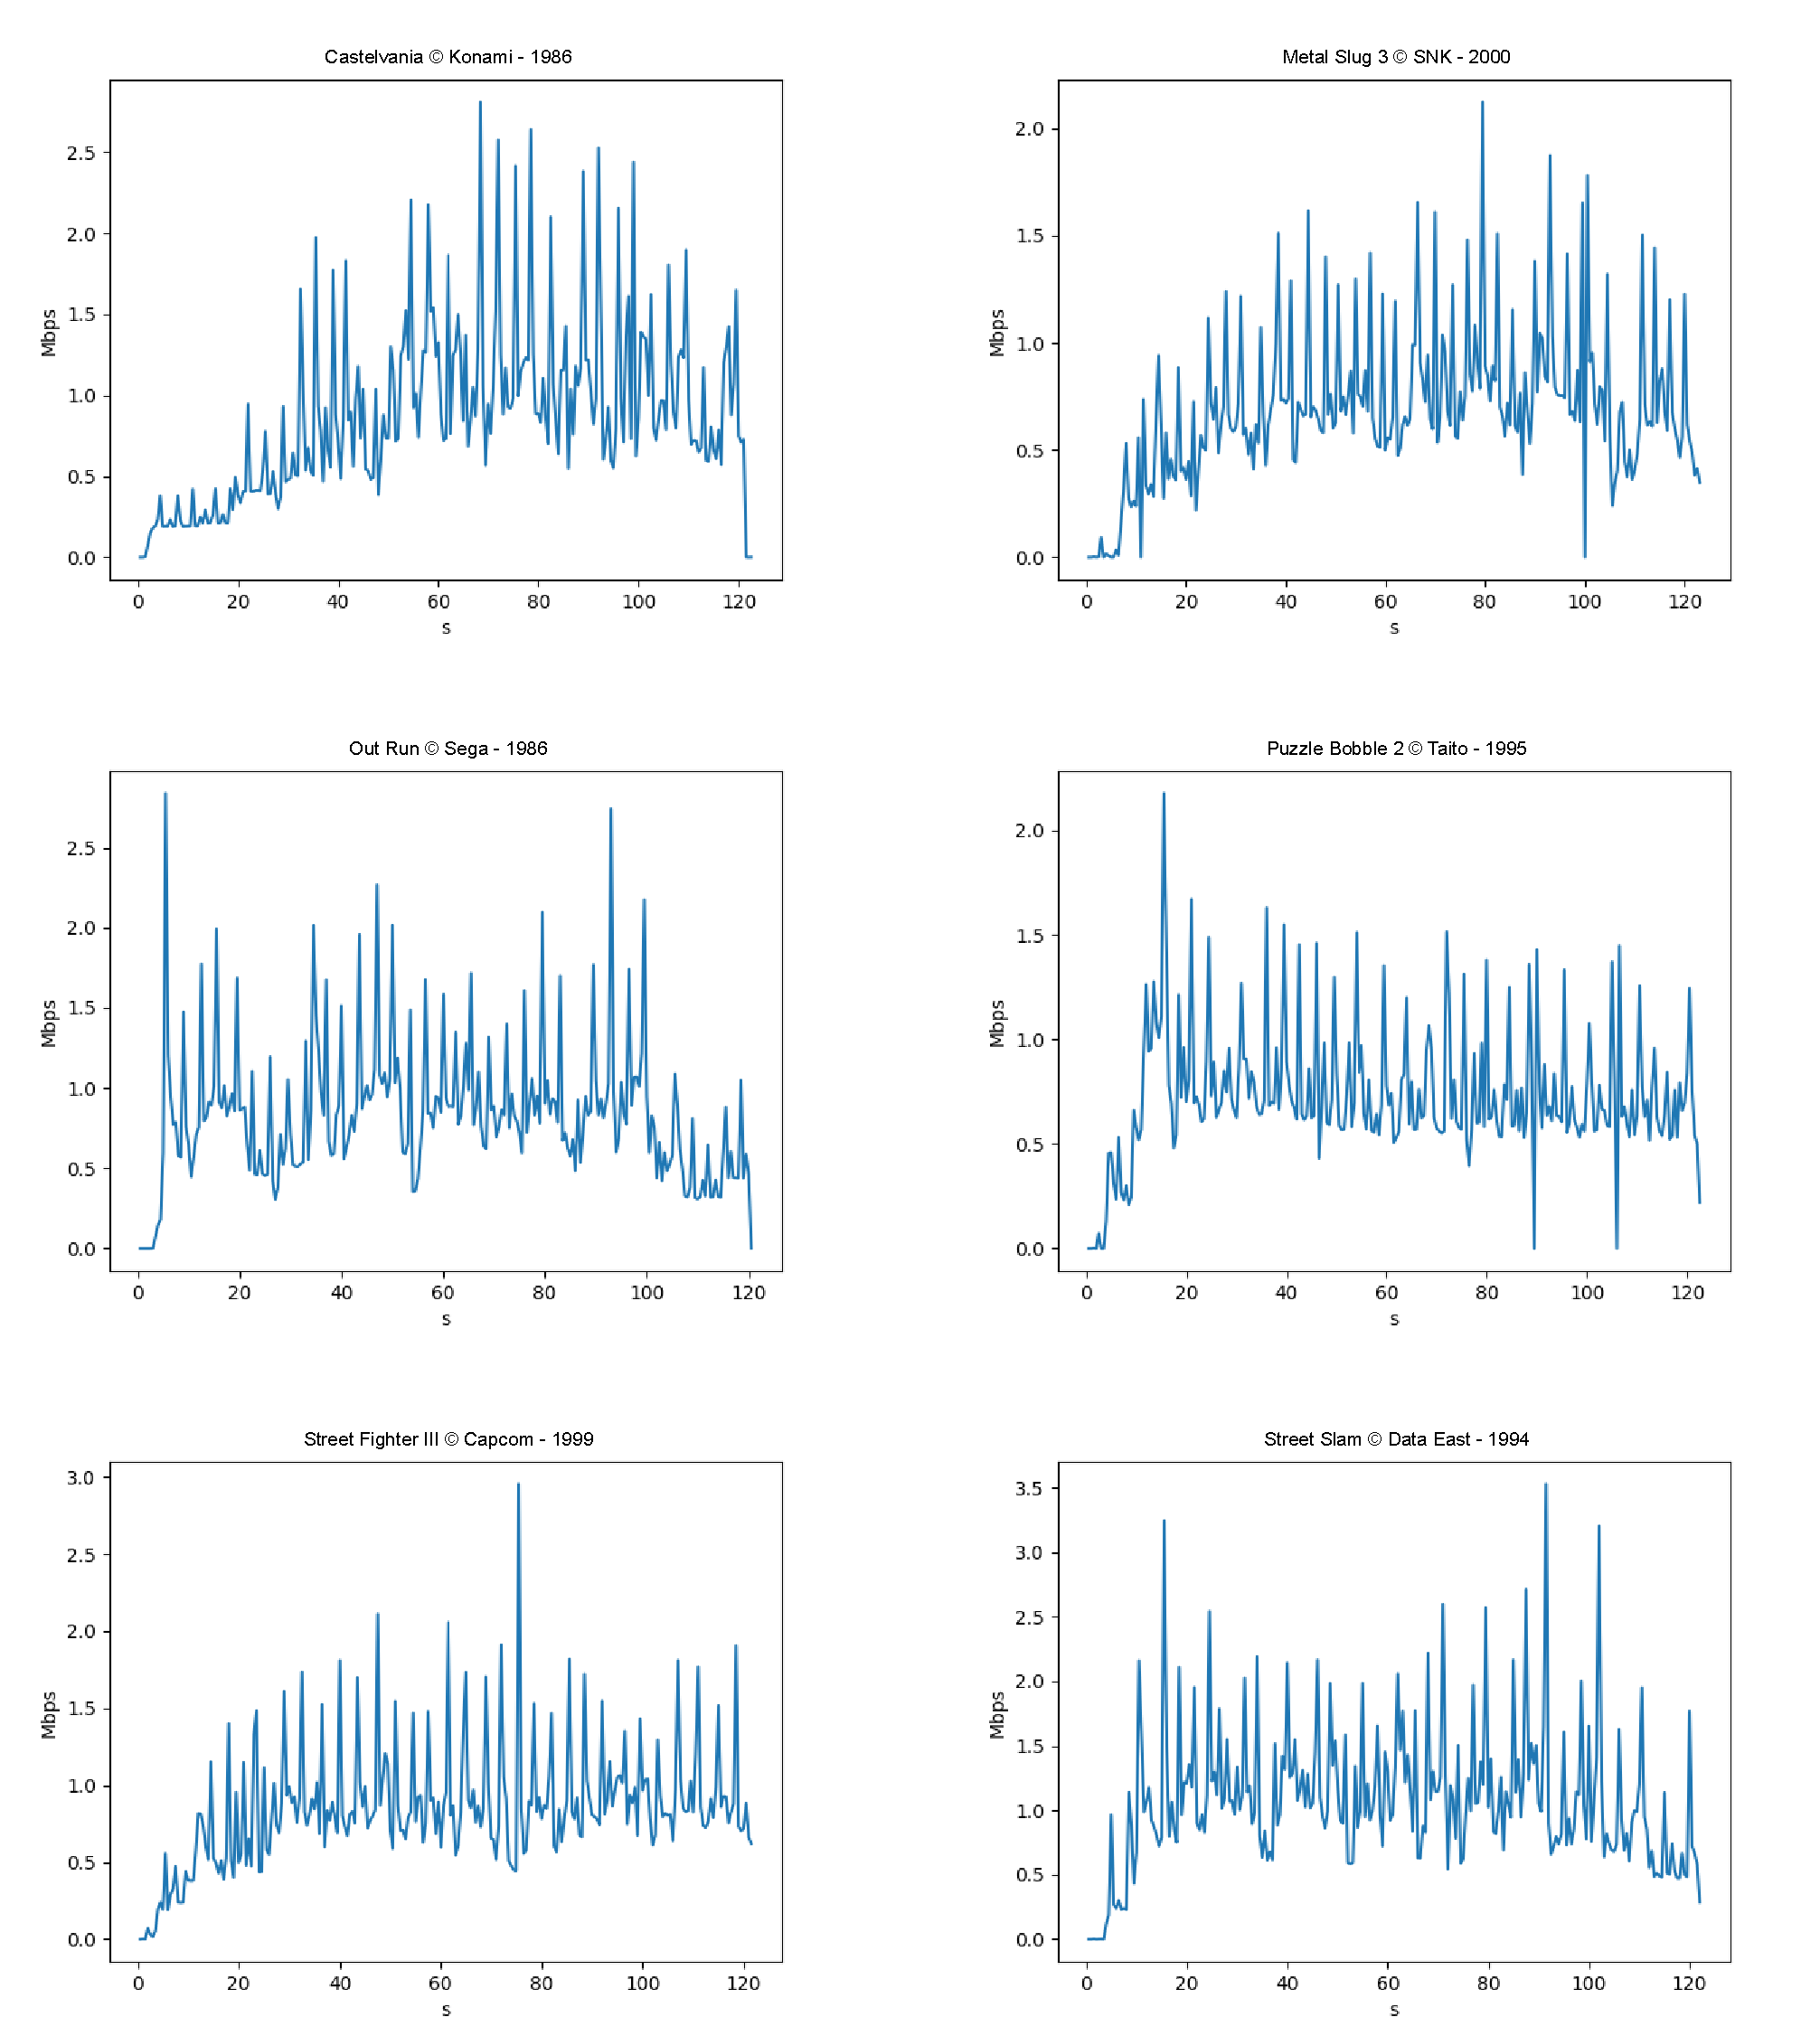
\includegraphics[width=\linewidth]{immagini/bandwidth}
	\caption{Bit-rate richiesto per vari tipi di giochi}	
	\label{fig:bandwidth}
\end{figure}




\section{Bit-rate richiesto}
Acaihjichai hcaih ciahci \parencite{wahab_ahmad_martini_schormans_2021}. Forse più questo \parencite{sun_2019}.